\documentclass[10pt,oneside]{article}
\usepackage[T1]{fontenc}
\usepackage[utf8]{inputenc}
% \usepackage{lmodern}
%\usepackage[adobe-utopia,uppercase=upright,greeklowercase=upright]{mathdesign}
\usepackage[adobe-utopia]{mathdesign}
%\usepackage{minionpro}
% \usepackage{pifont}
% \usepackage{amssymb}
\usepackage{amsmath}
\usepackage[francais]{babel}
% \usepackage[francais]{varioref}
\usepackage[dvips]{graphicx}

\usepackage{framed}
\usepackage[normalem]{ulem}
\usepackage{fancyhdr}
\usepackage{titlesec}
\usepackage{vmargin}
\usepackage{longtable}

\usepackage{ifthen}


%\usepackage{epsfig}
\usepackage{subfig}

\usepackage{multirow}
\usepackage{multicol} % Portions de texte en colonnes
\usepackage{flafter}%floatants après la référence



\usepackage{color}
\usepackage{colortbl}


\definecolor{gris25}{gray}{0.75}
\definecolor{bleu}{RGB}{18,33,98}
\definecolor{bleuf}{RGB}{42,94,171}
\definecolor{bleuc}{RGB}{231,239,247}
\definecolor{rougef}{RGB}{185,18,27}
\definecolor{rougec}{RGB}{255,230,231}
\definecolor{vertf}{RGB}{103,126,82}
\definecolor{vertc}{RGB}{220,255,191}

\newenvironment{rem}[1][\hsize]%
{%
    \def\FrameCommand
    {%
\rotatebox{90}{\textit{\textsf{Remarque}}} 
        {\color{bleuf}\vrule width 3pt}%
        \hspace{0pt}%must no space.
        \fboxsep=\FrameSep\colorbox{bleuc}%
    }%
    \MakeFramed{\hsize#1\advance\hsize-\width\FrameRestore}%
}%
{\endMakeFramed}%


\newenvironment{savoir}[1][\hsize]%
{%
    \def\FrameCommand
    {%
\rotatebox{90}{\textit{\textsf{Savoir}}} 
        {\color{bleuf}\vrule width 3pt}%
        \hspace{0pt}%must no space.
        \fboxsep=\FrameSep\colorbox{bleuc}%
    }%
    \MakeFramed{\hsize#1\advance\hsize-\width\FrameRestore}%
}%
{\endMakeFramed}%

\newenvironment{prob}[1][\hsize]%
{%
    \def\FrameCommand%
    {%
\rotatebox{90}{\textit{\textsf{ Problématique}}} 
        {\color{rougef}\vrule width 3pt}%
        \hspace{0pt}%must no space.
        \fboxsep=\FrameSep\colorbox{rougec}%
    }%
    \MakeFramed{\hsize#1\advance\hsize-\width\FrameRestore}%
}%
{\endMakeFramed}%

\newenvironment{obj}[1][\hsize]%
{%
    \def\FrameCommand%
    {%
\rotatebox{90}{\textit{\textsf{ $\;$}}} 
        {\color{rougef}\vrule width 3pt}%
        \hspace{0pt}%must no space.
        \fboxsep=\FrameSep\colorbox{rougec}%
    }%
    \MakeFramed{\hsize#1\advance\hsize-\width\FrameRestore}%
}%
{\endMakeFramed}%

\newenvironment{defi}[1][\hsize]%
{%
    \def\FrameCommand%
    {%
\rotatebox{90}{\textit{\textsf{Définition\\}}} 
        {\color{bleuf}\vrule width 3pt}%
        \hspace{0pt}%must no space.
        \fboxsep=\FrameSep\colorbox{bleuc}%
    }%
    \MakeFramed{\hsize#1\advance\hsize-\width\FrameRestore}%
}%
{\endMakeFramed}%


\newenvironment{hypo}[1][\hsize]%
{%
    \def\FrameCommand%
    {%
\rotatebox{90}{\textit{\textsf{Hypothèse\\}}} 
        {\color{bleuf}\vrule width 3pt}%
        \hspace{0pt}%must no space.
        \fboxsep=\FrameSep\colorbox{bleuc}%
    }%
    \MakeFramed{\hsize#1\advance\hsize-\width\FrameRestore}%
}%
{\endMakeFramed}%


\newenvironment{prop}[1][\hsize]%
{%
    \def\FrameCommand%
    {%
\rotatebox{90}{\textit{\textsf{Propriété\\}}} 
        {\color{bleuf}\vrule width 3pt}%
        \hspace{0pt}%must no space.
        \fboxsep=\FrameSep\colorbox{bleuc}%
    }%
    \MakeFramed{\hsize#1\advance\hsize-\width\FrameRestore}%
}%
{\endMakeFramed}%

\newenvironment{props}[1][\hsize]%
{%
    \def\FrameCommand%
    {%
\rotatebox{90}{\textit{\textsf{Propriétés\\}}} 
        {\color{bleuf}\vrule width 3pt}%
        \hspace{0pt}%must no space.
        \fboxsep=\FrameSep\colorbox{bleuc}%
    }%
    \MakeFramed{\hsize#1\advance\hsize-\width\FrameRestore}%
}%
{\endMakeFramed}%

\newenvironment{exemple}[1][\hsize]%
{%
    \def\FrameCommand%
    {%
\rotatebox{90}{\textit{\textsf{Exemple\\}}} 
        {\color{vertf}\vrule width 3pt}%
        \hspace{0pt}%must no space.
        \fboxsep=\FrameSep\colorbox{vertc}%
    }%
    \MakeFramed{\hsize#1\advance\hsize-\width\FrameRestore}%
}%
{\endMakeFramed}%

\newenvironment{resultat}[1][\hsize]%
{%
    \def\FrameCommand%
    {%
\rotatebox{90}{\textit{\textsf{Résultat\\}}} 
        {\color{rougef}\vrule width 3pt}%
        \hspace{0pt}%must no space.
        \fboxsep=\FrameSep\colorbox{rougec}%
    }%
    \MakeFramed{\hsize#1\advance\hsize-\width\FrameRestore}%
}%
{\endMakeFramed}%

\newenvironment{methode}[1][\hsize]%
{%
    \def\FrameCommand%
    {%
\rotatebox{90}{\textit{\textsf{Méthode\\}}} 
        {\color{rougef}\vrule width 3pt}%
        \hspace{0pt}%must no space.
        \fboxsep=\FrameSep\colorbox{rougec}%
    }%
    \MakeFramed{\hsize#1\advance\hsize-\width\FrameRestore}%
}%
{\endMakeFramed}%

\newenvironment{theo}[1][\hsize]%
{%
    \def\FrameCommand%
    {%
\rotatebox{90}{\textit{\textsf{Théorème\\}}} 
        {\color{rougef}\vrule width 3pt}%
        \hspace{0pt}%must no space.
        \fboxsep=\FrameSep\colorbox{rougec}%
    }%
    \MakeFramed{\hsize#1\advance\hsize-\width\FrameRestore}%
}%
{\endMakeFramed}%

\newenvironment{warn}[1][\hsize]%
{%
    \def\FrameCommand%
    {%
\rotatebox{90}{\textit{\textsf{Attention\\}}} 
        {\color{rougef}\vrule width 3pt}%
        \hspace{0pt}%must no space.
        \fboxsep=\FrameSep\colorbox{rougec}%
    }%
    \MakeFramed{\hsize#1\advance\hsize-\width\FrameRestore}%
}%
{\endMakeFramed}%

% \usepackage{pstricks}
%\usepackage{minitoc}
% \setcounter{minitocdepth}{4}

\setcounter{tocdepth}{2}

% \mtcselectlanguage{french} 

%\usepackage{draftcopy}% "Brouillon"
% \usepackage{floatflt}
\usepackage{psfrag}
%\usepackage{listings} % Permet d'insérer du code de programmation
\renewcommand{\baselinestretch}{1.2}

% Changer la numérotation des figures :
% ------------------------------------
% \makeatletter
% \renewcommand{\thefigure}{\ifnum \c@section>\z@ \thesection.\fi
%  \@arabic\c@figure}
% \@addtoreset{figure}{section}
% \makeatother
 


%%%%%%%%%%%%
% Définition des vecteurs %
%%%%%%%%%%%%
 \newcommand{\vect}[1]{\overrightarrow{#1}}

%%%%%%%%%%%%
% Définition des torseusr %
%%%%%%%%%%%%

 \newcommand{\torseur}[1]{%
\left\{{#1}\right\}
}

\newcommand{\torseurcin}[3]{%
\left\{\mathcal{#1} \left(#2/#3 \right) \right\}
}

\newcommand{\torseurstat}[3]{%
\left\{\mathcal{#1} \left(#2\rightarrow #3 \right) \right\}
}

 \newcommand{\torseurc}[8]{%
%\left\{#1 \right\}=
\left\{
{#1}
\right\}
 = 
\left\{%
\begin{array}{cc}%
{#2} & {#5}\\%
{#3} & {#6}\\%
{#4} & {#7}\\%
\end{array}%
\right\}_{#8}%
}

 \newcommand{\torseurcol}[7]{
\left\{%
\begin{array}{cc}%
{#1} & {#4}\\%
{#2} & {#5}\\%
{#3} & {#6}\\%
\end{array}%
\right\}_{#7}%
}

 \newcommand{\torseurl}[3]{%
%\left\{\mathcal{#1}\right\}_{#2}=%
\left\{%
\begin{array}{l}%
{#1} \\%
{#2} %
\end{array}%
\right\}_{#3}%
}

 \newcommand{\vectv}[3]{%
\vect{V\left( {#1} \in {#2}/{#3}\right)}
}


\newcommand{\vectf}[2]{%
\vect{R\left( {#1} \rightarrow {#2}\right)}
}

\newcommand{\vectm}[3]{%
\vect{\mathcal{M}\left( {#1}, {#2} \rightarrow {#3}\right)}
}


 \newcommand{\vectg}[3]{%
\vect{\Gamma \left( {#1} \in {#2}/{#3}\right)}
}

 \newcommand{\vecto}[2]{%
\vect{\Omega\left( {#1}/{#2}\right)}
}
% }$$\left\{\mathcal{#1} \right\}_{#2} =%
% \left\{%
% \begin{array}{c}%
%  #3 \\%
%  #4 %
% \end{array}%
% \right\}_{#5}}

%  ------------------------------------------
% | Modification du formatage des sections : | 
%  ------------------------------------------

% Grands titres :
% ---------------

\newcommand{\titre}[1]{%
\begin{center}
      \bigskip
      \rule{\textwidth}{1pt}
      \par\vspace{0.1cm}
      
      \textbf{\large #1}
      \par\rule{\textwidth}{1pt}
    \end{center}
    \bigskip
  }

% Supprime le numéro du chapitre dans la numérotation des sections:
% -----------------------------------------------------------------
\makeatletter
\renewcommand{\thesection}{\@arabic\c@section}
\makeatother


% \titleformat{\chapter}[display]
% {\normalfont\Large\filcenter}
% {}
% {1pc}
% {\titlerule[1pt]
%   \vspace{1pc}%
%   \Huge}[\vspace{1ex}%
% \titlerule]


%%%% Chapitres Comme PY Pechard %%%%%%%%%
% numéro du chapitre
\DeclareFixedFont{\chapnumfont}{OT1}{phv}{b}{n}{80pt}
% pour le mot « Chapitre »
\DeclareFixedFont{\chapchapfont}{OT1}{phv}{m}{it}{40pt}
% pour le titre
\DeclareFixedFont{\chaptitfont}{T1}{phv}{b}{n}{25pt}

\definecolor{gris}{gray}{0.75}
\titleformat{\chapter}[display]%
	{\sffamily}%
	{\filleft\chapchapfont\color{gris}\chaptertitlename\
	\\
	\vspace{12pt}
	\chapnumfont\thechapter}%
	{16pt}%
	{\filleft\chaptitfont}%
	[\vspace{6pt}\titlerule\titlerule\titlerule]

%%%%  Fin Chapitres Comme PY Pechard %%%%%%%%%


% Section, subsection, subsubsection sans serifs :
% % ----------------------------------------------

% \makeatletter
% \renewcommand{\section}{\@startsection{section}{0}{0mm}%
% {\baselineskip}{.3\baselineskip}%
% {\normalfont\sffamily\Large\textbf}}%
% \makeatother

\makeatletter
\renewcommand{\@seccntformat}[1]{{\textcolor{bleu}{\csname
the#1\endcsname}\hspace{0.5em}}}
\makeatother

\makeatletter
\renewcommand{\section}{\@startsection{section}{1}{\z@}%
                       {-4ex \@plus -1ex \@minus -.4ex}%
                       {1ex \@plus.2ex }%
                       {\normalfont\Large\sffamily\bfseries}}%
\makeatother
 
\makeatletter
\renewcommand{\subsection}{\@startsection {subsection}{2}{\z@}
                          {-3ex \@plus -0.1ex \@minus -.4ex}%
                          {0.5ex \@plus.2ex }%
                          {\normalfont\large\sffamily\bfseries}}
\makeatother
 
\makeatletter
\renewcommand{\subsubsection}{\@startsection {subsubsection}{3}{\z@}
                          {-2ex \@plus -0.1ex \@minus -.2ex}%
                          {0.2ex \@plus.2ex }%
                          {\normalfont\large\sffamily\bfseries}}
\makeatother
 
\makeatletter             
\renewcommand{\paragraph}{\@startsection{paragraph}{4}{\z@}%
                                    {-2ex \@plus-.2ex \@minus .2ex}%
                                    {0.1ex}%               
{\normalfont\sffamily\bfseries}}
\makeatother
 
\makeatletter
\renewcommand{\subparagraph}{\@startsection{subparagraph}{5}{\z@}%
                                       {-2ex \@plus-.1ex \@minus .2ex}%
                                       {0.1ex}%
				    {\normalfont\normalsize\sffamily\bfseries}}
\makeatletter
% \makeatletter
% \renewcommand{\subsection}{\@startsection{subsection}{1}{2mm}%
% {\baselineskip}{.3\baselineskip}%
% {\normalfont\sffamily\large\textbf}}%
% \makeatother
% 
% \makeatletter
% \renewcommand{\subsubsection}{\@startsection{subsubsection}{2}{4mm}%
% {\baselineskip}{.15\baselineskip}%
% {\normalfont\sffamily\large\textbf}}%
% \makeatother
% 
% \makeatletter
% \renewcommand{\paragraph}{\@startsection{paragraph}{3}{6mm}%
% {\baselineskip}{.15\baselineskip}%
% {\normalfont\sffamily\large\textbf}}%
% \makeatother
 
\setcounter{secnumdepth}{4}


%  --------
% | Marges |
%  --------


% \setmarginsrb{2.5cm}{1.5cm}{2.5cm}{2cm}{1cm}{1cm}{1cm}{1cm}
\setmarginsrb{1.5cm}{1cm}{1cm}{1.5cm}{1cm}{1cm}{1cm}{1cm}

% Changer les marges localement :
% -----------------------------
\newenvironment{changemargin}[2]{\begin{list}{}{%
\setlength{\topsep}{0pt}%
\setlength{\leftmargin}{0pt}%
\setlength{\rightmargin}{0pt}%
\setlength{\listparindent}{\parindent}%
\setlength{\itemindent}{\parindent}%
\setlength{\parsep}{0pt plus 1pt}%
\addtolength{\leftmargin}{#1}%
\addtolength{\rightmargin}{#2}%
}\item }{\end{list}}



\usepackage{pst-solides3d}
\usepackage{titletoc}
\titlecontents{chapter}[+3pc]
  {\addvspace{10pt}\sffamily\bfseries}
{\contentslabel[{\pscirclebox[fillstyle=solid,fillcolor=gray!25,
linecolor=gray!25,framesep=4pt]{\textcolor{white}{\thecontentslabel}}}]{2.5pc}}
  {}
  {\dotfill \normalfont\thecontentspage\ }

\titlecontents{section}[3pc]
  {\addvspace{2pt}\sffamily}
  {\contentslabel[\thecontentslabel]{1.8pc}}
  {}
  {\dotfill \normalfont\thecontentspage\ }

\titlecontents{subsection}[5pc]
  {\addvspace{2pt}\sffamily}
  {\contentslabel[\thecontentslabel]{1.8pc}}
  {}
  {\dotfill \normalfont\thecontentspage\ }

\titlecontents{subsubsection}[8pc]
  {\addvspace{2pt}\sffamily}
  {\contentslabel[\thecontentslabel]{3pc}}
  {}
  {\dotfill \normalfont\thecontentspage\ }
%{\;\titlerule\;\normalfont\thecontentspage\ }

\titlecontents{paragraph}[9pc]
  {\addvspace{2pt}\sffamily}
  {\contentslabel[\thecontentslabel]{3.5pc}}
  {}
  {\dotfill \normalfont\thecontentspage\ }





%Si le boolen xp est vrai : compilation pour xabi
%Sinon compilation Damien
\newboolean{xp}
\setboolean{xp}{true}

\newboolean{prof}
\setboolean{prof}{false}

\def\xxtitre{\ifthenelse{\boolean{xp}}{
CI 3 -- CIN : Étude du comportement cinématique des systèmes}{
}}

\def\xxsoustitre{\ifthenelse{\boolean{xp}}{
Chapitre 5 -- Cinématique du solide indéformable}{
}}


\def\xxauteur{\ifthenelse{\boolean{xp}}{
\noindent 2013 -- 2014 \\
Xavier \textsc{Pessoles}}{
}}


\def\xxpied{\ifthenelse{\boolean{xp}}{
CI 3 : CIN -- Cours \\
Ch 5 : Cinématique du solide -- \ifthenelse{\boolean{prof}}{P}{E}%
}{
}}

\usepackage[%
    pdftitle={CIN : Cinématique du solide},
    pdfauthor={Xavier Pessoles},
    colorlinks=true,
    linkcolor=blue,
    citecolor=magenta]{hyperref}


\usepackage{pifont}
\sloppy
\hyphenpenalty 10000


\begin{document}






% \makeatletter \let\ps@plain\ps@empty \makeatother
%% DEBUT DU DOCUMENT
%% =================




%------------- En tetes et Pieds de Pages ------------


\pagestyle{fancy}
\ifthenelse{\boolean{xp}}{%
\renewcommand{\headrulewidth}{0pt}}{%
\renewcommand{\headrulewidth}{0.2pt}} %pour mettre le trait en haut
%\renewcommand{\headrulewidth}{0.2pt}

\fancyhead{}
\fancyhead[L]{%
\ifthenelse{\boolean{xp}}{%
\noindent\begin{minipage}[c]{2.6cm}%

\includegraphics[width=2cm]{png/logo_ptsi.png}%
\end{minipage}%
}{%
\footnotesize{\textit{\textsf{Lycée François Premier}}}
}}

\ifthenelse{\boolean{xp}}{%
\fancyhead[C]{\rule{12cm}{.5pt}}}{
}


\fancyhead[R]{%
\noindent\begin{minipage}[c]{3cm}
\begin{flushright}
\footnotesize{\textit{\textsf{Sciences Industrielles \\ de l'ingénieur}}}%
\end{flushright}
\end{minipage}
}


\ifthenelse{\boolean{xp}}{%
\fancyhead[C]{\rule{12cm}{.5pt}}}{
}

\renewcommand{\footrulewidth}{0.2pt}

\fancyfoot[C]{\footnotesize{\bfseries \thepage}}
\fancyfoot[L]{%
\begin{minipage}[c]{.2\linewidth}
\noindent\footnotesize{{\xxauteur}}
\end{minipage}
\ifthenelse{\boolean{xp}}{}{%
\begin{minipage}[c]{.15\linewidth}

\includegraphics[width=2cm]{png/logoCC.png}
\end{minipage}}
}


\fancyfoot[R]{\footnotesize{\xxpied}}



\begin{center}
 \Large\textsc{\xxtitre}

\end{center}

\begin{center}
 \large\textsc{\xxsoustitre}
\end{center}

\begin{center}
 \Large\textsc{Exercice d'application}
\end{center}

\vspace{.25cm}

\subsection*{Etude d'une centrifugeuse à 2 degrés de liberté \cite{cite1}}

\vspace{.25cm}

\begin{minipage}[c]{.45\linewidth}
\begin{center}
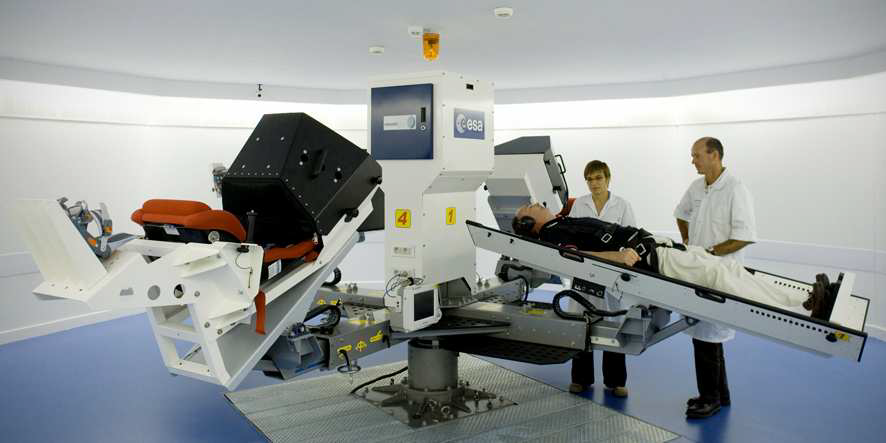
\includegraphics[height=4cm]{png/centrifugeuse_1}

\textit{Centrifugeuse humaine développée par le CNRS / MEDES } 

\end{center}
\end{minipage} \hfill
\begin{minipage}[c]{.45\linewidth}
\begin{center}
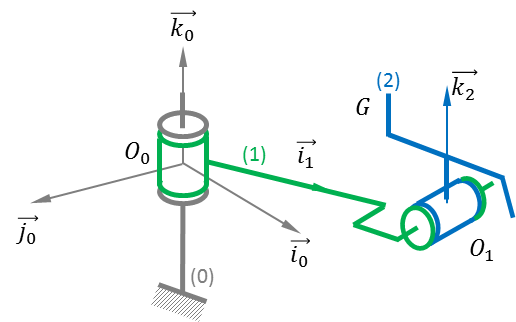
\includegraphics[height=4cm]{png/centrifugeuse_2}

\textit{Modélisation cinématique} 
\end{center}
\end{minipage}


\vspace{.25cm}


Le paramétrage de la centrifugeuse est donnée ci dessous : 


\begin{minipage}[c]{.45\linewidth}
\begin{center}
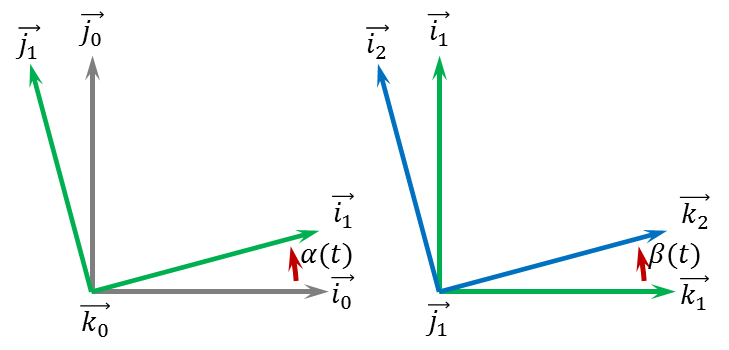
\includegraphics[height=3cm]{png/centrifugeuse_3}
\end{center}
\end{minipage}\hfill
\begin{minipage}[c]{.45\linewidth}
Les paramètres constants du système sont les suivants : 
\begin{itemize}%[$\bullet$]
\item $\vect{O_0O_1} = a \vect{i_1}$;
\item $\vect{O_1G} = b \vect{i_2} + c \vect{k_2}$.
\end{itemize}
\end{minipage}

\vspace{.25cm}


\subparagraph{}
\textit{Donner la trajectoire du point $G$ dans le repère $\mathcal{R}_0$.}
\ifthenelse{\boolean{prof}}{
\begin{corrige}
La trajectoire du point $G$ dans le repère $\mathcal{R}_0$  est donnée par le vecteur :
$$
\vect{O_0 G}(t)  = \vect{O_0O_1} + \vect{O_1G}
= a \vect{i_1} +  b \vect{i_2} + c \vect{k_2}
$$

Il faut alors projeter les vecteurs dans $\mathcal{R}_0$ : 
\begin{eqnarray*}
\vect{O_0 G}(t) &=& a \left(\cos\alpha(t) \vect{i_0} + \sin\alpha(t) \vect{j_0} \right) 
+ b \left(\cos\beta(t) \vect{i_1} - \sin\beta(t) \vect{k_1} \right) 
+ c\left(\cos\beta(t) \vect{k_1} + \sin\beta(t)\vect{i_1}\right)\\
&=& a \left(\cos\alpha(t) \vect{i_0} + \sin\alpha(t) \vect{j_0} \right) 
+ b \left(\cos\beta(t) \left(\cos\alpha(t) \vect{i_0} + \sin\alpha(t) \vect{j_0} \right) - \sin\beta(t) \vect{k_0} \right) \\
&& + c\left(\cos\beta(t) \vect{k_0} + \sin\beta(t)  \left(\cos\alpha(t) \vect{i_0} + \sin\alpha(t) \vect{j_0} \right) \right)\\
&=& \left[ \begin{array}{c} 
a \cos\alpha(t) + b \cos\beta(t) \cos\alpha(t) +c \sin\beta(t)\cos\alpha(t)\\
a \sin\alpha(t) + b \cos\beta(t) \sin\alpha(t) +c \sin\beta(t)\sin\alpha(t) \\
- b\sin\beta(t) + c\cos\beta(t)
\end{array}\right]_{\mathcal{R}_0}
\end{eqnarray*}

On a ainsi l'équation paramétrique de la position du point $G$.

\end{corrige}
}{}


\subparagraph{}
\textit{Calculer $\vectv{O_0}{S_1}{S_0}$.}

\subparagraph{}
\textit{Calculer $\vectv{O_1}{S_2}{S_1}$.}

\subparagraph{}
\textit{Calculer $\vectv{O_1}{S_1}{S_0}$.}
\ifthenelse{\boolean{prof}}{
\begin{corrige}


\textbf{Méthode 1 -- }
Par définition, 
$$
\vectv{O_1}{S_1}{S_0} 
= \left[\dfrac{d\vect{O_0O_1}(t)}{dt}\right]_{\mathcal{R}_0}
= \left[\dfrac{d \left(a \vect{i_1}\right) }{dt}\right]_{\mathcal{R}_0}
= a \left[\dfrac{d  \vect{i_1} }{dt}\right]_{\mathcal{R}_0}
$$

On a :
\begin{eqnarray*}
\left[\dfrac{d  \vect{i_1} }{dt}\right]_{\mathcal{R}_0}
&=&\left[\dfrac{d \left(\cos\alpha(t)\vect{i_0}+\sin\alpha(t)\vect{j_0} \right)}{dt}\right]_{\mathcal{R}_0}
=\left[\dfrac{d  \cos\alpha(t)\vect{i_0}}{dt}\right]_{\mathcal{R}_0}
+\left[\dfrac{d  \sin\alpha(t)\vect{j_0} }{dt}\right]_{\mathcal{R}_0}\\
& = & 
\dfrac{d \cos\alpha(t)}{dt} \vect{i_0}  
+\cos\alpha(t)\underbrace{\left[\dfrac{d  \vect{i_0}}{dt}\right]_{\mathcal{R}_0}}_{\vect{0}}
+\dfrac{d \sin\alpha(t)}{dt} \vect{i_0}  
+\sin(t)\underbrace{\left[\dfrac{d  \vect{j_0}}{dt}\right]_{\mathcal{R}_0}}_{\vect{0}}\\
& = & -\dot{\alpha}(t)\sin\alpha(t) \vect{i_0}   + \dot{\alpha}(t)\cos\alpha(t) \vect{j_0}  = 
\dot{\alpha}(t)\vect{j_1}
\end{eqnarray*}

Ainsi,
$$
\vectv{O_1}{S_1}{S_0} 
= \left[\begin{array}{c} 
-a\dot{\alpha}(t)\sin\alpha(t) \\
a \dot{\alpha}(t)\cos\alpha(t) \\
0 \end{array}\right]_{\mathcal{R}_0}
=\left[\begin{array}{c} 0 \\ a\dot{\alpha}(t) \\ 0\end{array}\right]_{\mathcal{R}_1}
$$

Dans les deux cas, $\vect{O_0O_1}(t)$ est dérivé par rapport $\mathcal{R}_0$ mais il s'exprime différemment dans $\mathcal{R}_0$ et $\mathcal{R}_1$ :
\begin{itemize}
\item $\vectv{O_1}{S_1}{S_0} = -a\dot{\alpha}(t)\sin\alpha(t) \vect{i_0}   + a\dot{\alpha}(t) \cos\alpha(t) \vect{j_0}$ : ici la base de \textbf{projection} et de \textbf{dérivation} est la base $\mathcal{B}_0$;
\item $\vectv{O_1}{S_1}{S_0} = a\dot{\alpha}(t)\vect{j_1}$ : ici la base de dérivation est la base $\mathcal{B}_0$ et la base de projection est $\mathcal{B}_1$.
\end{itemize}


\textbf{Méthode 2 -- Utilisation de la dérivation vectorielle.}

Calcul de $\vectv{O_1}{S_1}{S_0}$.

On rappelle que :
$$
\vectv{O_1}{S_1}{S_0} 
= a \left[\dfrac{d  \vect{i_1} }{dt}\right]_{\mathcal{R}_0}
$$

Le calcul de $\left[\dfrac{d  \vect{i_1} }{dt}\right]_{\mathcal{R}_0}$ peut donc être réalisé ainsi : 
$$ 
\left[\dfrac{d  \vect{i_1} }{dt}\right]_{\mathcal{R}_0} = 
\underbrace{\left[\dfrac{d  \vect{i_1} }{dt}\right]_{\mathcal{R}_1}}_{\vect{0}} + \vecto{S_1}{S_0}\wedge \vect{i_1}
=\dot{\alpha}\vect{k_0}  \wedge \vect{i_1}
=\dot{\alpha} \vect{j_1}
$$

Ainsi 
$$
\vectv{O_1}{S_1}{S_0} 
= a \dot{\alpha} \vect{j_1}
$$

\textbf{Méthode 3 -- }
Calcul de $\vectv{O_1}{S_1}{S_0}$.

$S_1$ et $S_0$ sont en liaison pivot de centre $O_0$, on a donc :  $\vectv{O_0}{S_1}{S_0}=\vect{0}$.

En conséquence, 
$$
\vectv{O_1}{S_1}{S_0} = \vectv{O_0}{S_1}{S_0} + \vect{O_1O_0}\wedge   \vecto{S_1}{S_0} = \vect{0} - a \vect{i_1} \wedge \left( \dot{\alpha}\vect{k_0} \right)
=a \dot{\alpha}\vect{j_1}
$$

\end{corrige}}{}


\subparagraph{}
\textit{Calculer $\vecto{S_1}{S_0}$, $\vecto{S_2}{S_1}$ et $\vecto{S_2}{S_0}$.}



\subparagraph{}
\textit{Calculer $\vectv{G}{S_2}{S_0}$.}
\ifthenelse{\boolean{prof}}{
\begin{corrige}

Calcul de $\vectv{G}{S_2}{S_0}$.
%On a :
%$$\vecto{S_2}{S_0}=\vecto{S_2}{S_1}+\vecto{S_1}{S_0} = \dot{\alpha}\vect{k_0} + \dot{\beta}\vect{j_1}  $$

%Par ailleurs, 
On a : 
$$\vectv{G}{S_2}{S_0} = \vectv{G}{S_2}{S_1} + \vectv{G}{S_1}{S_0} $$
Calculons $\vectv{G}{S_1}{S_0}$ :
$$
\vectv{G}{S_1}{S_0} 
= \vectv{O_1}{S_1}{S_0} + \vect{GO_1}\wedge\vecto{S_1}{S_0}
= a\dot{\alpha}\vect{j_1} - \left(b\vect{i_2} + c\vect{k_2}\right) \wedge\left( \dot{\alpha} \vect{k_0}\right)
$$
$$
\vectv{G}{S_1}{S_0} 
= a\dot{\alpha}\vect{j_1}  + b\dot{\alpha} \sin(\beta+\pi/2) \vect{j_1} + c \dot{\alpha}\sin\beta\vect{j_1}
= \dot{\alpha} \left(a+b \cos\beta + c \sin\beta\right) \vect{j_1} 
$$

Par ailleurs calculons $\vectv{G}{S_2}{S_1}$ :
$$\vectv{G}{S_2}{S_1} = \vectv{O_1}{S_2}{S_1} + \vect{GO_1}\wedge \vecto{S_2}{S_1}
=-\left(b\vect{i_2}+c\vect{k_2}\right) \wedge \left(\dot{\beta}\vect{j_1}\right)
=-\dot{\beta}\left(b\vect{k_2}-c\vect{i_2} \right)
$$

Au final, 
$$\vectv{G}{S_2}{S_0} = \dot{\alpha} \left(a+b \cos\beta + c \sin\beta\right) \vect{j_1} 
-\dot{\beta}\left(b\vect{k_2}-c\vect{i_2} \right)
$$

Il est aussi possible de calculer $\vectv{G}{S_2}{S_0}$ ainsi : 
$$\vectv{G}{S_2}{S_0} = \left[\dfrac{d \vect{O_0G}}{dt}\right]_{\mathcal{R}_0}$$ 

\end{corrige}}{}



\subparagraph{}
\textit{Calculer $\vectg{O_1}{S_2}{S_0}$.}
\ifthenelse{\boolean{prof}}{
\begin{corrige}
\end{corrige}}{}


\subparagraph{}
\textit{Calculer $\vectg{G}{S_2}{S_0}$.}
\ifthenelse{\boolean{prof}}{
\begin{corrige}
\end{corrige}}{}


\begin{thebibliography}{2}
\bibitem[1]{cite1} Centrifugeuse humaine -- CNRS Photothèque/Sébastien Godefroy et MEDES, \textit{Avio et Tiger}, \url{http://www.medes.fr/home_fr/fiche-centrifugeuse/mainColumnParagraphs/0/document/Presentation%20centrifugeuse%2018.12.07.pdf}.
\end{thebibliography}
\end{document}

